\section{Suddivisione del lavoro}
I componenti del gruppo dovranno rivestire ognuno dei ruoli come specificato nella sezione XXXXXX
\subsection{Analisi}
Nella fase di \textbf{Analisi} ciascun componente dovrà ricoprire i seguenti ruoli e per la quantità di ore specificate:

\begin{table}[H]
	\centering
	\begin{tabular}{|l|c|c|c|c|c|c|c|}
		\hline
		\textbf{Nominativo} & 
		\multicolumn{6}{c|}{\textbf{Ore per ruolo}} & 
		\textbf{Ore totali} \\
		& Re & Am & An & Pj & Pr & Ve & \\
		\hline
		Nicola Dal Maso & & 8 & 9 & & & 10 & 27 \\
		Lorenzo Ferrarin & & 7 & 12 & & & 10 & 29 \\
		Beatrice Guerra & 19 & & & & & 10 & 29 \\
		Marco Ponchia & & & 15 & & & 12 & 27 \\
		Tommaso Rosso & & 4 & 24 & & & & 28 \\
		Alice V. Sasso & & 8 & 20 & & & & 28 \\
		Mattia Zecchinato & 18 & & 10 & & & & 28 \\
		\hline
	\end{tabular}
	\caption{Ore per componente, fase di Analisi}
\end{table}
I valori sono riassunti nel seguente grafico, che rappresenta in maniera visiva per quante ore un membro ricoprirà un determinato ruolo.
\begin{figure}[H]
	\centering
	\scalebox{0.6}{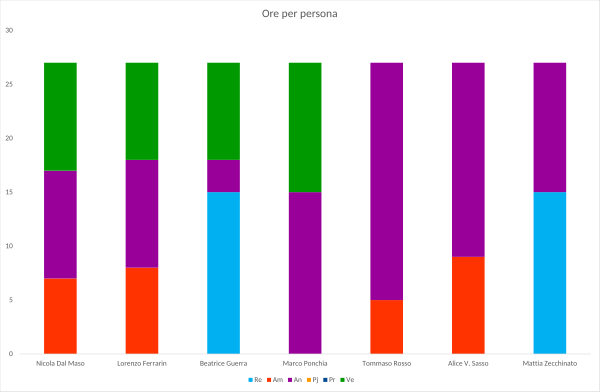
\includegraphics{img_suddlavoro/AA.png}}
	\caption{Ore per componente, fase di Analisi}
\end{figure}


\subsection{Analisi di dettaglio}
Nella fase di \textbf{Analisi di dettaglio} ciascun componente dovrà ricoprire i seguenti ruoli e per la quantità di ore specificate:

\begin{table}[H]
	\centering
	\begin{tabular}{|l|c|c|c|c|c|c|c|}
		\hline
		\textbf{Nominativo} & 
		\multicolumn{6}{c|}{\textbf{Ore per ruolo}} & 
		\textbf{Ore totali} \\
		& Re & Am & An & Pj & Pr & Ve & \\
		\hline
		Nicola Dal Maso & & 8 & 9 & & & 10 & 27 \\
		Lorenzo Ferrarin & & 7 & 12 & & & 10 & 29 \\
		Beatrice Guerra & 19 & & & & & 10 & 29 \\
		Marco Ponchia & & & 15 & & & 12 & 27 \\
		Tommaso Rosso & & 4 & 24 & & & & 28 \\
		Alice V. Sasso & & 8 & 20 & & & & 28 \\
		Mattia Zecchinato & 18 & & 10 & & & & 28 \\
		\hline
	\end{tabular}
	\caption{Ore per componente, fase di Analisi di dettaglio}
\end{table}
I valori sono riassunti nel seguente grafico, che rappresenta in maniera visiva per quante ore un membro ricoprirà un determinato ruolo.
\begin{figure}[H]
	\centering
	\scalebox{0.6}{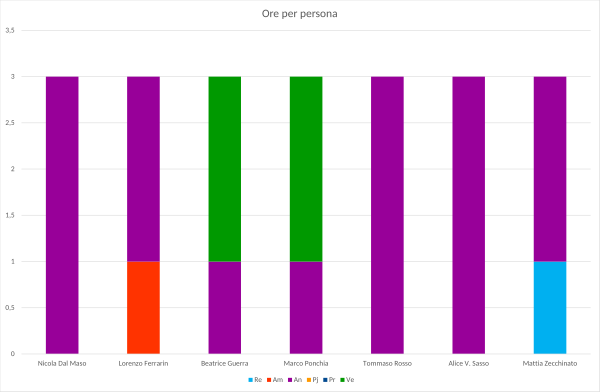
\includegraphics{img_suddlavoro/AD.png}}
	\caption{Ore per componente, fase di Analisi di dettaglio}
\end{figure}

\subsection{Progettazione Architetturale}
Nella fase di \textbf{Progettazione Architetturale} ciascun componente dovrà ricoprire i seguenti ruoli e per la quantità di ore specificate:

\begin{table}[H]
	\centering
	\begin{tabular}{|l|c|c|c|c|c|c|c|}
		\hline
		\textbf{Nominativo} & 
		\multicolumn{6}{c|}{\textbf{Ore per ruolo}} & 
		\textbf{Ore totali} \\
		& Re & Am & An & Pj & Pr & Ve & \\
		\hline
		Nicola Dal Maso & & 8 & 9 & & & 10 & 27 \\
		Lorenzo Ferrarin & & 7 & 12 & & & 10 & 29 \\
		Beatrice Guerra & 19 & & & & & 10 & 29 \\
		Marco Ponchia & & & 15 & & & 12 & 27 \\
		Tommaso Rosso & & 4 & 24 & & & & 28 \\
		Alice V. Sasso & & 8 & 20 & & & & 28 \\
		Mattia Zecchinato & 18 & & 10 & & & & 28 \\
		\hline
	\end{tabular}
	\caption{Ore per componente, fase di Progettazione Architetturale}
\end{table}
I valori sono riassunti nel seguente grafico, che rappresenta in maniera visiva per quante ore un membro ricoprirà un determinato ruolo.
\begin{figure}[H]
	\centering
	\scalebox{0.6}{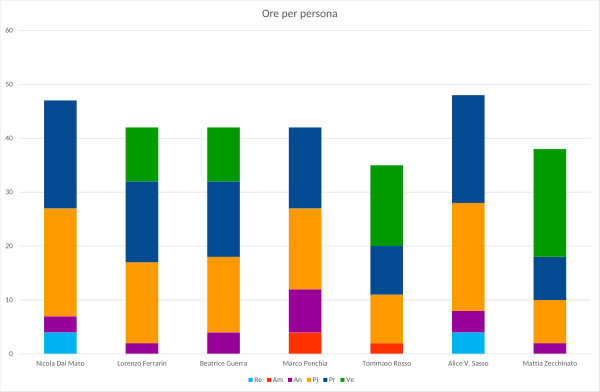
\includegraphics{img_suddlavoro/PA.png}}
	\caption{Ore per componente, fase di Progettazione Architetturale}
\end{figure}

\subsection{Progettazione di dettaglio e codifica}
Nella fase di \textbf{Progettazione di dettaglio e codifica} ciascun componente dovrà ricoprire i seguenti ruoli e per la quantità di ore specificate:

\begin{table}[H]
	\centering
	\begin{tabular}{|l|c|c|c|c|c|c|c|}
		\hline
		\textbf{Nominativo} & 
		\multicolumn{6}{c|}{\textbf{Ore per ruolo}} & 
		\textbf{Ore totali} \\
		& Re & Am & An & Pj & Pr & Ve & \\
		\hline
		Nicola Dal Maso & & 8 & 9 & & & 10 & 27 \\
		Lorenzo Ferrarin & & 7 & 12 & & & 10 & 29 \\
		Beatrice Guerra & 19 & & & & & 10 & 29 \\
		Marco Ponchia & & & 15 & & & 12 & 27 \\
		Tommaso Rosso & & 4 & 24 & & & & 28 \\
		Alice V. Sasso & & 8 & 20 & & & & 28 \\
		Mattia Zecchinato & 18 & & 10 & & & & 28 \\
		\hline
	\end{tabular}
	\caption{Ore per componente, fase di Progettazione di dettaglio e codifica}
\end{table}
I valori sono riassunti nel seguente grafico, che rappresenta in maniera visiva per quante ore un membro ricoprirà un determinato ruolo.
\begin{figure}[H]
	\centering
	\scalebox{0.6}{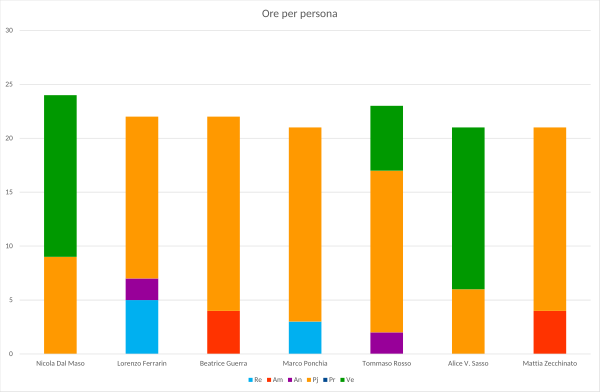
\includegraphics{img_suddlavoro/PD.png}}
	\caption{Ore per componente, fase di Progettazione di dettaglio e codifica}
\end{figure}

\subsection{Codifica}
Nella fase di \textbf{Codifica} ciascun componente dovrà ricoprire i seguenti ruoli e per la quantità di ore specificate:

\begin{table}[H]
	\centering
	\begin{tabular}{|l|c|c|c|c|c|c|c|}
		\hline
		\textbf{Nominativo} & 
		\multicolumn{6}{c|}{\textbf{Ore per ruolo}} & 
		\textbf{Ore totali} \\
		& Re & Am & An & Pj & Pr & Ve & \\
		\hline
		Nicola Dal Maso & & 8 & 9 & & & 10 & 27 \\
		Lorenzo Ferrarin & & 7 & 12 & & & 10 & 29 \\
		Beatrice Guerra & 19 & & & & & 10 & 29 \\
		Marco Ponchia & & & 15 & & & 12 & 27 \\
		Tommaso Rosso & & 4 & 24 & & & & 28 \\
		Alice V. Sasso & & 8 & 20 & & & & 28 \\
		Mattia Zecchinato & 18 & & 10 & & & & 28 \\
		\hline
	\end{tabular}
	\caption{Codifica}
\end{table}
I valori sono riassunti nel seguente grafico, che rappresenta in maniera visiva per quante ore un membro ricoprirà un determinato ruolo.
\begin{figure}[H]
	\centering
	\scalebox{0.6}{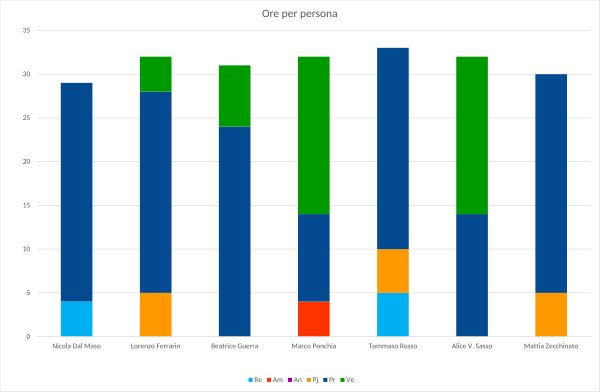
\includegraphics{img_suddlavoro/C.png}}
	\caption{Ore per componente, fase di Codifica}
\end{figure}

\subsection{Verifica e Validazione}
Nella fase di \textbf{Verifica e Validazione} ciascun componente dovrà ricoprire i seguenti ruoli e per la quantità di ore specificate:

\begin{table}[H]
	\centering
	\begin{tabular}{|l|c|c|c|c|c|c|c|}
		\hline
		\textbf{Nominativo} & 
		\multicolumn{6}{c|}{\textbf{Ore per ruolo}} & 
		\textbf{Ore totali} \\
		& Re & Am & An & Pj & Pr & Ve & \\
		\hline
		Nicola Dal Maso & & 8 & 9 & & & 10 & 27 \\
		Lorenzo Ferrarin & & 7 & 12 & & & 10 & 29 \\
		Beatrice Guerra & 19 & & & & & 10 & 29 \\
		Marco Ponchia & & & 15 & & & 12 & 27 \\
		Tommaso Rosso & & 4 & 24 & & & & 28 \\
		Alice V. Sasso & & 8 & 20 & & & & 28 \\
		Mattia Zecchinato & 18 & & 10 & & & & 28 \\
		\hline
	\end{tabular}
	\caption{Ore per componente, fase di Verifica e Validazione}
\end{table}
I valori sono riassunti nel seguente grafico, che rappresenta in maniera visiva per quante ore un membro ricoprirà un determinato ruolo.
\begin{figure}[H]
	\centering
	\scalebox{0.6}{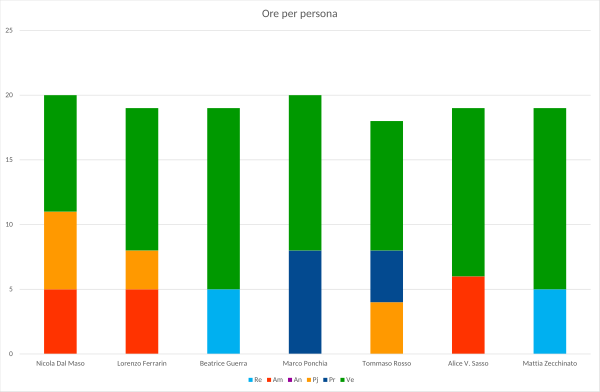
\includegraphics{img_suddlavoro/VV.png}}
	\caption{Ore per componente, fase di Verifica e Validazione}
\end{figure}

\subsection{Totale}
\subsubsection{Ore totali con investimento}
Le ore totali, comprese quelle investire in analisi, divise per componente durante il progetto saranno le seguenti:

\begin{table}[H]
	\centering
	\begin{tabular}{|l|c|c|c|c|c|c|c|}
		\hline
		\textbf{Nominativo} & 
		\multicolumn{6}{c|}{\textbf{Ore per ruolo}} & 
		\textbf{Ore totali} \\
		& Re & Am & An & Pj & Pr & Ve & \\
		\hline
		Nicola Dal Maso & & 8 & 9 & & & 10 & 27 \\
		Lorenzo Ferrarin & & 7 & 12 & & & 10 & 29 \\
		Beatrice Guerra & 19 & & & & & 10 & 29 \\
		Marco Ponchia & & & 15 & & & 12 & 27 \\
		Tommaso Rosso & & 4 & 24 & & & & 28 \\
		Alice V. Sasso & & 8 & 20 & & & & 28 \\
		Mattia Zecchinato & 18 & & 10 & & & & 28 \\
		\hline
	\end{tabular}
	\caption{Ore totali per componente compresa l'analisi non rendicontata}
\end{table}
I valori sono riassunti nel seguente grafico, che rappresenta in maniera visiva per quante ore un membro ricoprirà un determinato ruolo.
\begin{figure}[H]
	\centering
	\scalebox{0.6}{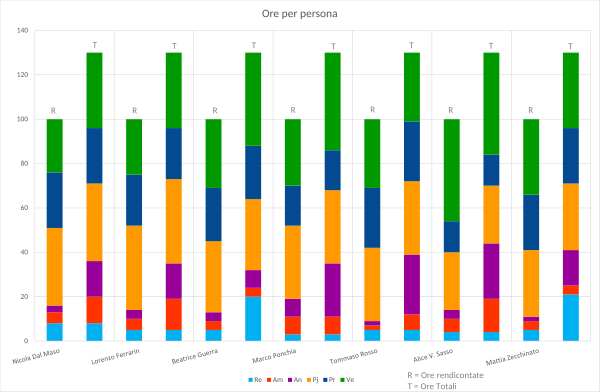
\includegraphics{img_suddlavoro/TOT.png}}
	\caption{Ore per componente, fase di Verifica e Validazione}
\end{figure}

\subsubsection{Ore rendicontate}
Le ore totali rendicontatee divise per componente durante il progetto saranno le seguenti:

\begin{table}[H]
	\centering
	\begin{tabular}{|l|c|c|c|c|c|c|c|}
		\hline
		\textbf{Nominativo} & 
		\multicolumn{6}{c|}{\textbf{Ore per ruolo}} & 
		\textbf{Ore totali} \\
		& Re & Am & An & Pj & Pr & Ve & \\
		\hline
		Nicola Dal Maso & & 8 & 9 & & & 10 & 27 \\
		Lorenzo Ferrarin & & 7 & 12 & & & 10 & 29 \\
		Beatrice Guerra & 19 & & & & & 10 & 29 \\
		Marco Ponchia & & & 15 & & & 12 & 27 \\
		Tommaso Rosso & & 4 & 24 & & & & 28 \\
		Alice V. Sasso & & 8 & 20 & & & & 28 \\
		Mattia Zecchinato & 18 & & 10 & & & & 28 \\
		\hline
	\end{tabular}
	\caption{Ore totali rendicontate}
\end{table}
I valori sono riassunti nel seguente grafico, che rappresenta in maniera visiva per quante ore un membro ricoprirà un determinato ruolo.
\begin{figure}[H]
	\centering
	\scalebox{0.6}{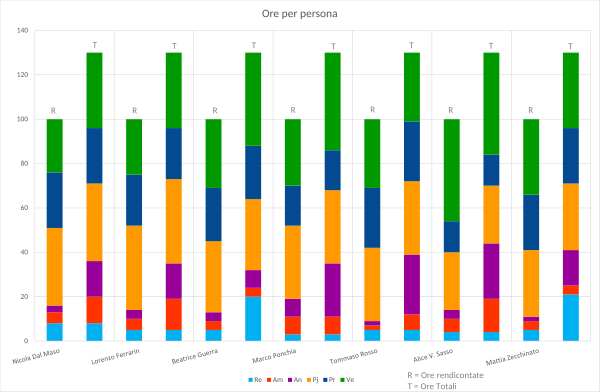
\includegraphics{img_suddlavoro/TOT.png}}
	\caption{Ore per componente, fase di Verifica e Validazione}
\end{figure}





